\documentclass[uplatex,dvipdfmx,11pt,a4paper]{jsarticle} %11pt A4用紙出力

\usepackage{okumacro} % jsclassesに同梱のパッケージ いろんなマクロがある
% 和文の仮想ボディがアレ
\usepackage{otf}
% 欧文フォントのサイズ指定がアレ
\usepackage[T1]{fontenc}
\usepackage{lmodern}
% 用紙サイズの扱いがアレ
\usepackage{bxpapersize}
% 空白文字を含む画像を読み込めるようにする
\usepackage{grffile}
% 余白設定
\usepackage[top=20mm, bottom=25mm, left=20mm, right=20mm]{geometry}

\usepackage[dvipdfmx]{hyperref} % ハイパーリンクつき文章にする
\usepackage{pxjahyper}
\usepackage{xcolor}
\hypersetup{
    colorlinks=false,
    citebordercolor=green,
    linkbordercolor=red,
    urlbordercolor=cyan,
}

\usepackage[dvipdfmx]{graphicx} %画像読み込み
\usepackage[dvipdfmx]{color} %png画像が表示されないとき
\usepackage{amsmath} %数式
\usepackage{bm} % 太字、ベクトル
\usepackage{textcomp} % 特殊文字
\usepackage{siunitx} % SI単位系
\usepackage{paralist} % 改行しない箇条書きを可能にする 
\usepackage{url} %url
\usepackage{multirow} %表 縦結合
\usepackage{multicol}
\usepackage{subfigure} %副番号
\usepackage{fancyhdr} %ヘッダ フッタ
\usepackage{float}
\usepackage{tikz}
\usepackage[RPvoltages]{circuitikz}
\usepackage{cases}

\usepackage{here} %画像配置
    \pagestyle{fancy}
    \lhead{}
    \chead{}
    \rhead{\thepage}
    \lfoot{}
    \cfoot{}
    \rfoot{}
    \renewcommand{\headrulewidth}{0pt}

\usepackage{minted}
\usepackage{listings,jlisting} %日本語のコメントアウトをする場合jlistingが必要
\usepackage{txfonts}

% solarized
\definecolor{base}{gray}{0} %black
\definecolor{comment}{rgb}{0.52,0.60,0.00} %green
\definecolor{string}{rgb}{0.83,0.21,0.51} %magenta
\definecolor{keyword1}{rgb}{0.15,0.55,0.82} %blue
\definecolor{keyword2}{rgb}{0.80,0.29,0.09} %orange
\definecolor{keyword3}{rgb}{0.71,0.54,0.00} %yellow
\definecolor{keyword4}{rgb}{0.42,0.44,0.77} %violet[f:id:e8l:20151129232557p:plain][f:id:e8l:20151129232557p:plain][f:id:e8l:20151129232557p:plain]

\lstset
{
    basicstyle={\ttfamily\color{base}\scriptsize},%コードの基本書式
    keywordstyle=[1]{\color{keyword1}\textbf},%キーワード1のスタイル
    keywordstyle=[2]{\color{keyword2}\textbf},%キーワード2のスタイル
    keywordstyle=[3]{\color{keyword3}\textbf},%キーワード3のスタイル
    keywordstyle=[4]{\color{keyword4}\textbf},%キーワード4のスタイル
    commentstyle={\gtfamily\scriptsize\color{comment}},%コメントのスタイル
    stringstyle={\gtfamily\scriptsize\color{string}},%文字列のスタイル
    numbers=left,%行番号は左
    stepnumber=1,%一行ずつ行番号をふる
    numberstyle={\sffamily\scriptsize},%行番号の書式
    xleftmargin=0zw, %左余白
    xrightmargin=0zw,%右余白
    tabsize=4,%タブの空白数
    % frame=single,フレームの書式
    frame={tb},
    % frameround=tttt,角を丸めるかどうか tで丸める
    breaklines=true,%長くなったら途中で改行
    captionpos=t,%タイトルの位置
    breakindent=10pt,%改行されたときの送り幅
    showstringspaces=false,%文字列中の半角スペースを表示させない
    lineskip=-1pt%通常の文章より行送りを狭くする
}

% mktitleを調整
\usepackage{mdframed}
\makeatletter
\newcommand{\subtitle}[1]{\def\@subtitle{#1}}
\newcommand{\institute}[1]{\def\@institute{#1}}
\renewcommand{\maketitle}{
  \begin{mdframed}[roundcorner=10pt]
    {\small \@date}
    \vspace{-2.5ex}
    \begin{center}
      \textgt{\@subtitle}\\[0.25ex]
      {\Large \textgt{\@title}}
    \end{center}
    \vspace{-3.5ex}
    \begin{flushright}
      \@institute \hspace{0.5em} \@author
    \end{flushright}
  \end{mdframed}
}
\makeatother


\usepackage{problem}
\usepackage{pxpdfpages}
\usepackage{pdfpages}

\bibliographystyle{jIEEEtran}

\renewcommand{\listingscaption}{ソースコード}

\title{TCP/UDP通信とブロードキャスト(設計書)}
\subtitle{ネットワークプログラミング}
\author{情報工学課程 渡邉紘矢}
\institute{学籍番号:18122508}
\date{\today}

\begin{document}
\maketitle
% \includepdf{}
\setcounter{page}{1}

\section{共通して使用する定数値}
\begin{itemize}
    \item サーバー検索時の返り値
    
     プログラムの起動時にHEROパケットを送信 し、返事があるかどうかでサーバーが既に起動しているか、していないかを判断する。この結果の返り値として用い、主に可読性のために使用を検討している。
    \lstinputlisting[language=c, caption=サーバー検索時の返り値, label=sc:constant1]{src/constants/1}

    \item パケットのタイプ

         取得するパケットの種類は全部で6種類である。どの種類のパケットを作成するのか、どのパケットを受信したのかを判断するために用いる。
    \lstinputlisting[language=c, caption=パケットのタイプ, label=sc:constant2]{src/constants/2}

    \item UDP通信時に用いるタイムアウトの時間

         サーバー検索にはUDPを用いる。UDPはコネクションレスな通信であるため、相手に必ずパケットが届くことが保証されておらず、送信すれば返ってくるはずの返事が返ってこない場合がある。そのための、タイムアウトの時間を設定するために用いる。単位は秒である。
    \lstinputlisting[language=c, caption=UDP通信時に用いるタイムアウトの時間, label=sc:constant3]{src/constants/3}

    \item 各データのサイズ

         仕様書に従い、プログラム内で適切にバッファやデータ処理を行うために、各データのサイズを定義しておく。
    \lstinputlisting[language=c, caption=各データのサイズ, label=sc:constant4]{src/constants/4}

    \item 文字色と背景色のペアを表す定数値

         今回は、ncursesライブラリを用いて、端末制御を行う。ncursesでは、文字色と背景色のペアを定数値に登録し、その値を用いて色のペアを呼び出すことになる。その色を明確に呼び出せるように用いる。
    \lstinputlisting[language=c, caption=文字色と背景色のペアを表す定数値, label=sc:constant5]{src/constants/5}
\end{itemize}

\section{共通して使用する構造体}
\begin{itemize}
    \item ユーザの情報を格納する構造体

         ユーザ情報を格納するために、線形リストの構造を利用する。
        ユーザはソケット番号を用いて一意に特定することが可能であり、ソケット番号を用いてユーザ名を特定できるようにする。また、ユーザが途中で抜けることがあり、ユーザの情報を削除する際に、線形リストであれば1箇所のポインタを設定しなおすことで実現できる。
    \lstinputlisting[language=c, caption=ユーザの情報を格納する構造体, label=sc:struct1]{src/struct/1}

    \item パケットの構造

         送信するデータは、ヘッダとして4バイトの識別文字列を付加され、メッセージ本体とヘッダがスペースで区切られた文字列であるとする。この文字列が、以下のようなデータ構造になっているとして扱うと、受信したパケットのタイプ、メッセージ本体を扱いやすくできる。
    \lstinputlisting[language=c, caption=パケットの構造, label=sc:struct2]{src/struct/2}
\end{itemize}

\section{ウィンドウ作成用ソースコード({\tt window.c})}
{\tt window.c}には、以下のような定数値と関数を用意する。ここには、プロトタイプ宣言のみ記述することにする。
    \lstinputlisting[language=c, caption=window.cの実装, label=sc:window1]{src/window/1}

\begin{itemize}
    \item {\tt \#define SUBWIN\_LINES 5}

         メッセージを表示するメインウィンドウと、自分が送信したいメッセージを入力するサブウィンドウを用意する。
        そのサブウィンドウの行数を指定する。
        \newline
    \item {\tt static void init\_color\_pair()}

         以下の3種類の背景色と文字色のペアを登録する。
        \begin{itemize}
            \item 背景色:白 文字色:黒
            \item 背景色:白 文字色:緑
            \item 背景色:白 文字色:水色
        \end{itemize}
       \begin{description}
            \item[引数:] なし
            \item[返り値:] なし
            \newline
       \end{description}

    \item {\tt void create\_window(WINDOW **win\_main, WINDOW **win\_sub)}

         メインウィンドウとサブウィンドウを作成する。以下の初期設定が完了したウィンドウがセットされる。
        \begin{itemize}
            \item 日本語を表示出来るようにする
            \item 色を変更出来るようにする
            \item 使用する色を定義する
            \item 背景色を白、文字色を黒にする
            \item スクロールを許可する
        \end{itemize}
         \begin{description}
            \item[引数:] \ 

                \begin{itemize}
                    \item win\_main: 作成されたメインウィンドウ。受信したメッセージを表示するウィンドウになる。
                    \item win\_sub: 作成されたサブウィンドウ。ユーザのキーボード入力を表示するウィンドウになる。
                \end{itemize}
            \item[返り値:] なし
         \end{description}
\end{itemize}

\section{パケットの解析+作成用ソースコード({\tt packet.c})}
{\tt packet.c}には、以下のような関数を用意する。
    \lstinputlisting[language=c, caption=packet.cの実装, label=sc:packet1]{src/packet/1}

\begin{itemize}
    \item {\tt void create\_packet(char *Buffer, unsigned int type, char *message)}

         パケットの種類と、送信したいメッセージ本体からパケットを作成する。
        \begin{description}
            \item[引数:] \ 

                \begin{itemize}
                        \item Buffer: 作成されたパケット。セットされたデータをTCPやUDP通信で送信する。
                        \item type: 作成したいパケットの種類
                        \item message: 送信したいメッセージ本体
                \end{itemize}
            \item[返り値:] なし
            \newline
        \end{description}

    \item {\tt unsigned int analyze\_header(char *header)}

         パケットの種類を調べ、種類を表す整数値を返す。
        \begin{description}
            \item[引数:] \ 

                \begin{itemize}
                        \item header: 受信したパケットのヘッダ部分
                \end{itemize}
            \item[返り値:] パケットの種類を表す整数値
        \end{description}
\end{itemize}

\section{ユーザ情報へアクセスするための線形リストの実装({\tt linear\_lists.c})}
{\tt packet.c}には、以下のような変数と関数を用意する。
    \lstinputlisting[language=c, caption=linear\_lists.cの実装, label=sc:linear1]{src/linear_lists/1}
\begin{itemize}
    \item {\tt static member\_t head = NULL}

         線形リストの先頭を指すポインタ。線形リストにデータが無い時はNULL値になる。
        \newline
    \item {\tt static member\_t tail = NULL}

         線形リストの末尾を指すポインタ。線形リストにデータが無い時はNULL値になる。
        \newline
    \item {\tt static member\_t create\_member()}

         新たなユーザのデータを格納するために、動的に構造体分のメモリを確保し、そのポインタを返す。
        \begin{description}
            \item[引数:] なし
            \item[返り値:] 1人分のデータを格納する構造体へのポインタ
            \newline
        \end{description}

    \item {\tt member\_t get\_head\_from\_list()}

         線形リストの先頭を指すポインタを返す。
        \begin{description}
            \item[引数:] なし
            \item[返り値:] 線形リストの先頭を指すポインタ
            \newline
        \end{description}

    \item {\tt void add\_user\_to\_list(char *username, int sock)}

         ユーザの情報として、ユーザ名とソケット番号を格納し、線形リストの末尾に追加する。
        \begin{description}
            \item[引数:] \ 

                \begin{itemize}
                    \item username: ユーザの名前
                    \item sock: そのユーザとTCP通信を行うためのソケット番号
                \end{itemize}
            \item[返り値:] なし
            \newline
        \end{description}

    \item {\tt void delete\_user\_from\_list(int sock)}

         ソケット番号を用いて、ユーザを特定し、そのユーザ情報を線形リストから削除する。
        \begin{description}
            \item[引数:] \ 

                \begin{itemize}
                    \item sock: そのユーザとTCP通信を行うためのソケット番号
                \end{itemize}
            \item[返り値:] なし
        \end{description}
\end{itemize}

\section{共通で使用する関数のソースコード({\tt idobata\_common.c})}
{\tt idobata\_common.c}には、以下のような変数と関数を用意する。
\lstinputlisting[language=c, caption=idobata\_common.cの実装, label=sc:common1]{src/common/1}
\begin{itemize}
    \item {\tt char server\_addr[20]}

         サーバーを検索した結果、サーバーから返事があった時、そのサーバーのIPアドレスを格納するための変数。TCP通信においてコネクションを確立する際に用いる。
        \newline

    \item {\tt char user\_name[USERNAME\_LEN]} 

         JOINパケットを送信する際にユーザ名をメッセージ本体に含めるため、変数にセットしておく。
        \newline

    \item {\tt int search\_server(int port\_number)}

         ブロードキャストを行い、ネットワーク上にサーバーが存在するか調べる。タイムアウトを3回するまでパケットを再送する。3回の送信でサーバーが見つからなかった場合は0を返し、見つかった場合は即座に1を返す。
        \begin{description}
            \item[引数:] \ 

                \begin{itemize}
                    \item port\_number: サーバーが通信を待ち受けているポート番号
                \end{itemize}
            \item[返り値:] サーバーが見つかった時は1、見つからなかった時は0を返す
            \newline
        \end{description}

    \item {\tt void set\_server\_addr(char *addr)}

         サーバーのIPアドレスを変数に格納する。
        \begin{description}
            \item[引数:] \ 

                \begin{itemize}
                    \item addr: サーバーのIPアドレス
                \end{itemize}
            \item[返り値:] なし
            \newline
        \end{description}

    \item {\tt void get\_server\_addr(char *out)}

         記憶しているサーバーのIPアドレスを引数に指定された配列にセットする。
        \begin{description}
            \item[引数:] \ 

                \begin{itemize}
                    \item out: サーバーのIPアドレスがセットされる配列
                \end{itemize}
            \item[返り値:] なし
            \newline
        \end{description}

    \item {\tt void set\_user\_name(char *name)}

         ユーザ名を変数に格納する。
        \begin{description}
            \item[引数:] \ 

                \begin{itemize}
                    \item name: ユーザ名
                \end{itemize}
            \item[返り値:] なし
            \newline
        \end{description}

    \item {\tt void get\_user\_name(char *out)}

         記憶しているユーザ名を引数に指定された配列にセットする。
        \begin{description}
            \item[引数:] \ 

                \begin{itemize}
                    \item out: ユーザ名がセットされる配列
                \end{itemize}
            \item[返り値:] なし
            \newline
        \end{description}

    \item {\tt void show\_your\_msg(WINDOW *win, char *buf)}

         背景色を白、文字色を緑色として、右端揃えで文字列を表示する。
        \begin{description}
            \item[引数:] \ 

                \begin{itemize}
                    \item win: 文字列を表示するウィンドウ
                    \item buf: 表示したい文字列
                \end{itemize}
            \item[返り値:] なし
            \newline
        \end{description}

    \item {\tt void show\_others\_msg(WINDOW *win, char *buf)}

         背景色を白、文字色を水色として、左端揃えで文字列を表示する。
        \begin{description}
            \item[引数:] \ 

                \begin{itemize}
                    \item win: 文字列を表示するウィンドウ
                    \item buf: 表示したい文字列
                \end{itemize}
            \item[返り値:] なし
            \newline
        \end{description}

    \item {\tt int cnt\_jp(char *str)}

         受け取った文字列の中に含まれている日本語の文字数を数え、その文字数を返す。
        \begin{description}
            \item[引数:] \ 

                \begin{itemize}
                    \item str: 調査対象となる文字列
                \end{itemize}
            \item[返り値:] 含まれている日本語の文字数
        \end{description}
\end{itemize}

\section{クライアント用関数のソースコード({\tt idobata\_client.c})}
{\tt idobata\_client.c}には、以下のような変数と関数を用意する。
\lstinputlisting[language=c, caption=idobata\_client.cの実装, label=sc:client1]{src/client/1}

\begin{itemize}
    \item {\tt static WINDOW *win\_main, *win\_sub}

         メッセージを表示するメインウィンドウと、ユーザのキーボード入力を表示するサブウィンドウ
        \newline
    \item {\tt static void init(int port\_number, int *sock)}

         以下の順序でクライアントの初期設定を行う。
        \begin{enumerate}
            \item ウィンドウを作成する
            \item サーバーとTCP通信のコネクションを確立させる
            \item サーバーにJOINパケットを送信する
            \item サーバーとの通信に用いるソケット番号をsock変数にセットする
        \end{enumerate}
        \begin{description}
            \item[引数:] \ 

                \begin{itemize}
                        \item port\_number: サーバーのポート番号
                        \item sock: サーバーと通信するためのソケット番号
                \end{itemize}
            \item[返り値:] なし
            \newline
        \end{description}

    \item {\tt int join\_server(int port\_number)}

         サーバーとTCP通信のコネクションを確立させ、サーバーにJOINパケットを送信する。今後もサーバーと通信を行うので、そのソケット番号を返す。
        \begin{description}
            \item[引数:] \ 

                \begin{itemize}
                        \item port\_number: サーバーのポート番号
                \end{itemize}
            \item[返り値:] サーバーと通信するためのソケット番号
            \newline
        \end{description}

    \item {\tt void send\_msg\_from\_keyboard(int sock, char *p\_buf)}

         キーボード入力を受け取った文字列を用いてPOSTパケットを作成し、サーバーに送信する。
        \begin{description}
            \item[引数:] \ 

                \begin{itemize}
                        \item sock: サーバーとの通信に用いるソケット番号
                        \item p\_buf: キーボード入力を受け取った文字列
                \end{itemize}
            \item[返り値:] なし
        \end{description}
\end{itemize}

\section{サーバー用関数のソースコード({\tt idobata\_server.c})}
{\tt idobata\_client.c}には、以下のような定数値、変数と関数を用意する。
\lstinputlisting[language=c, caption=idobata\_server.cの実装, label=sc:server1]{src/server/1}
 
\begin{itemize}
    \item {\tt \#define FROM\_SERVER -1}

         サーバーがメッセージを転送する際には、メッセージ本体の先頭にユーザ名を付加してから送信する。そのため、ユーザ名を取得するためにソケット番号と一致するまで線形リストを走査する必要がある。この時、サーバーの情報は線形リストに含まれないため、転送ではなく、サーバーから直接メッセージを送信したい場合はソケット番号を-1とすることで上手く処理する。
        \newline

    \item {\tt static WINDOW *win\_main, *win\_sub}

         メッセージを表示するメインウィンドウと、ユーザのキーボード入力を表示するサブウィンドウ
        \newline

    \item {\tt fd\_set mask, readfds}

         selectを用いて通信やキーボード入力を監視するためのマスク(mask)と監視状況をセットする(readfds)変数
        \newline

    \item {\tt static int Max\_sd = 0}

         selectを用いて監視する値の最大値がセットされる
        \newline

    \item {\tt static void init(int port\_number, int *server\_udp\_sock, int *server\_tcp\_sock, int *client\_tcp\_sock)}

         サーバーの初期設定を行う。サーバーは各クライアントの接続を受け付け、各クライアントにメッセージを転送する役割を持つ。また、サーバーはサーバーとしてだけでなく、1つのクライアントとしても実行されるようになっている。それぞれの通信に用いるソケット番号が引数に指定された変数にセットされる。よってサーバーは以下の順序で初期化を行う。
        \begin{enumerate}
            \item ウィンドウを作製する
            \item UDPサーバーを初期化する
            \item TCPサーバーを初期化する
            \item クライアントを初期化し、サーバーに接続する
            \item 各ソケット番号を変数にセットする
        \end{enumerate}
        \begin{description}
            \item[引数:] \ 

                \begin{itemize}
                        \item port\_number: サーバーとして通信を待ち受けるポート番号
                        \item server\_udp\_sock: UDP通信を行うためのソケット番号
                        \item server\_tcp\_sock: クライアントがコネクション確立のために通信してくるのを待ち受けるソケット番号
                        \item client\_tcp\_sock: サーバーは同時にクライアントとしても実行されている。そのクライアントがサーバーと通信を行うためのソケット番号
                \end{itemize}
            \item[返り値:] なし
            \newline
        \end{description}

    \item {\tt void idobata\_server(int port\_number)}

         指定されたポート番号でサーバーを実行する。また同時に、そのサーバーに接続するクライアントも実行することで、サーバー兼クライアントとして振る舞う。
        \begin{description}
            \item[引数:] \ 

                \begin{itemize}
                        \item port\_number: サーバーとして通信を待ち受けるポート番号
                \end{itemize}
            \item[返り値:] なし
            \newline
        \end{description}

    \item {\tt static void recv\_udp\_packet(int udp\_sock)}

         UDPパケットを受信し、パケットの情報をもとにサーバーを検索しているクライアントに対して、HEREパケットを送信する。
        \begin{description}
            \item[引数:] \ 

                \begin{itemize}
                        \item udp\_sock: UDP通信に用いるためのソケット番号
                \end{itemize}
            \item[返り値:] なし
            \newline
        \end{description}

    \item {\tt static void recv\_msg\_from\_client()}

         クライアントからデータが届いているか確認し、受信できる相手からデータを受信する。届いたパケットの種類や内容に応じて以下のような分岐処理を行う。
        \begin{itemize}
            \item クライアントが切断したならユーザの登録情報を削除する
            \item 名前が登録されていない場合、JOINパケットを待ち、登録させる
            \item パケットの種類がPOSTだったらメッセージを転送する
            \item パケットの種類がQUITだったら、コネクションを切断し、ユーザの登録情報を削除する
        \end{itemize}
        \begin{description}
            \item[引数:] なし
            \item[返り値:] なし
            \newline
        \end{description}

    \item {\tt static void register\_username(member\_t user, ido\_packet\_t *packet)}

         パケットの種類がJOINだったら、パケットのメッセージ本体をユーザ名として登録する。
        また、新たにクライアントが参加したことを全クライアントに通知する。
        \begin{description}
            \item[引数:] \ 

                \begin{itemize}
                    \item user: ユーザ情報を格納している構造体へのポインタ
                    \item packet: 受信したパケットの構造体へのポインタ
                \end{itemize}
            \item[返り値:] なし
            \newline
        \end{description}

    \item {\tt static void delete\_user(char *user\_name, int sock)}

         クライアントがサーバーから切断したことを全クライアントに通知する。そのユーザのソケット番号をselectで監視する対象外とし、ユーザの情報を線形リストから削除する。
        \begin{description}
            \item[引数:] \ 

                \begin{itemize}
                        \item user\_name: 削除するユーザ情報のユーザ名
                        \item sock: 削除するユーザと通信するためのソケット番号
                \end{itemize}
            \item[返り値:] なし
            \newline
        \end{description}

    \item {\tt static void transfer\_message(char *message, char *from\_user\_name, int from\_sock)}

         転送するメッセージ本体の先頭にユーザ名を付加し、MESSAGEパケットを作成する。もとの送信者であるクライアント以外にそのパケットを送信する。
        \begin{description}
            \item[引数:] \ 

                \begin{itemize}
                        \item message: 転送するメッセージ本体
                        \item from\_user\_name: メッセージをサーバに送信してきたクライアントのユーザ名
                        \item from\_sock: メッセージをサーバに送信してきたクライアントのソケット番号
                \end{itemize}
            \item[返り値:] なし
            \newline
        \end{description}

    \item {\tt static void setMax\_sd(int num)}

         selectを実行する際に、監視する値の最大値+1を指定する必要がある。監視する最大値はクライアントとコネクションを確立するごとに変化することが考えられ、この関数を用いて常に最大値がセットされるようにする。
        \begin{description}
            \item[引数:] \ 

                \begin{itemize}
                    \item num: selectで監視する値
                \end{itemize}
            \item[返り値:] なし
        \end{description}
    
\end{itemize}

\section{井戸端会議エントリポイントのソースコード({\tt idobata.c})}
{\tt idobata.c}には、以下のような定数値、変数と関数を用意する。
\lstinputlisting[language=c, caption=idobata.cの実装, label=sc:idobata1]{src/idobata/1}

\begin{itemize}
    \item {\tt \#define DEFAULT\_PORT 50001}

         デフォルトのポート番号を指定する。実行時引数にポート番号が指定されなければポート番号として50001を用いる。
        \newline

    \item {\tt extern char *optarg}
    \item {\tt extern int optind, opterr, optopt}

         実行時引数にオプション指定を行うために予め宣言しておく変数
        \newline

    \item{\tt int main(int argc, char *argv[])}

         エントリポイント。以下の順序でクライアント、もしくはサーバーの動作へ分岐する。
        \begin{enumerate}
            \item 実行時引数のオプションを解析し、各値をセットする
            \item サーバがネットワーク内に存在するか検索する
            \item サーバが存在すれば、クライアントとして実行する。いなければ、サーバーとして実行する。
            \newline
        \end{enumerate}

    \item {\tt void help\_message(char *script\_name)}

         プログラムの使い方を表示する。
        \begin{description}
            \item[引数:] \ 

                \begin{itemize}
                    \item script\_name: プログラム実行時の実行ファイル名
                \end{itemize}
            \item[返り値:] なし
        \end{description}
\end{itemize}

\section{ヘッダファイル({\tt idobata.h})}
以上をまとめると、ヘッダファイルに記述する内容は以下のようになる。

\lstinputlisting[language=c, caption=idobata.h, label=sc:idobata2]{src/idobata/2}

\section{フローチャート}
プログラムの主要な部分のフローチャートを以下に示す。

\begin{figure}[H]
\centering
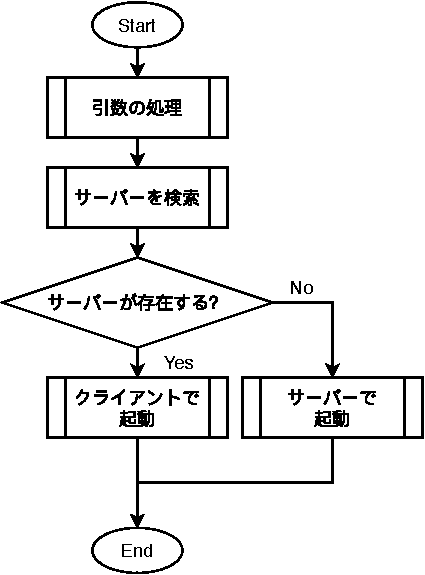
\includegraphics[]{figures/flow/1.pdf}
\caption{エントリポイントのフローチャート}
\label{fg:entry}
\end{figure}

\begin{figure}[H]
\centering
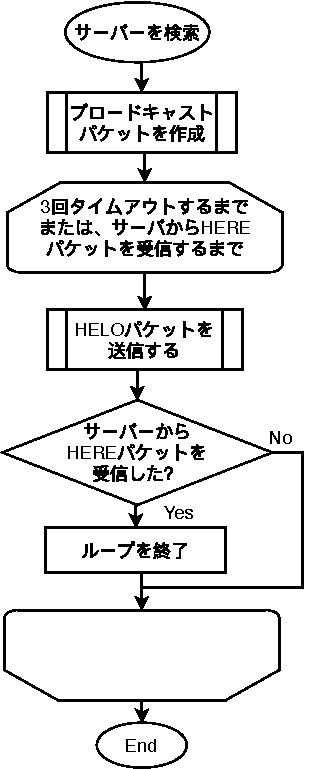
\includegraphics[]{figures/flow/2.pdf}
\caption{サーバー検索時のフローチャート}
\label{fg:search}
\end{figure}

\begin{figure}[H]
\centering
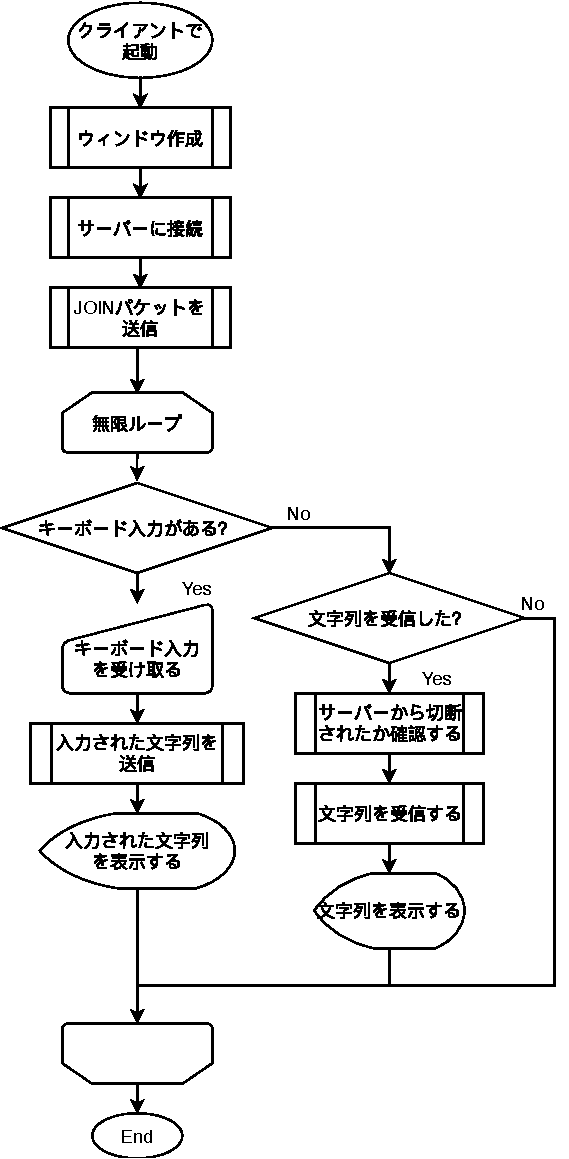
\includegraphics[]{figures/flow/3.pdf}
\caption{クライアントのフローチャート}
\label{fg:client}
\end{figure}

\begin{figure}[H]
\centering
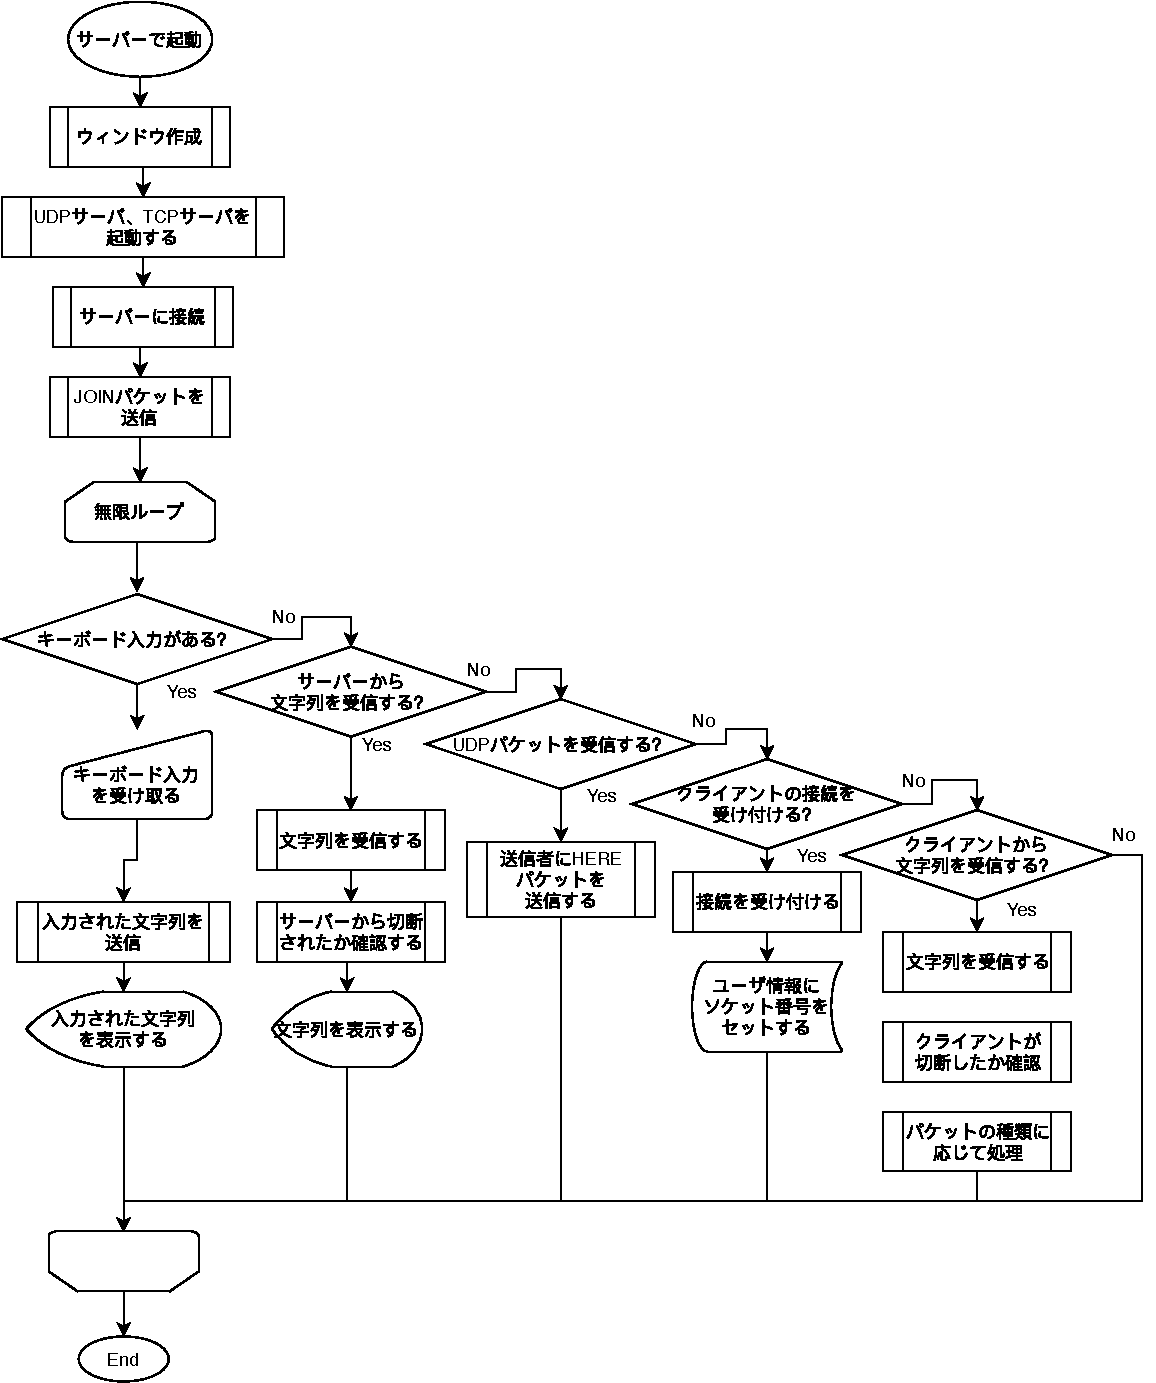
\includegraphics[width=\hsize]{figures/flow/4.pdf}
\caption{サーバーのフローチャート}
\label{fg:server}
\end{figure}

\section{クライアントからの不定期なデータ処理}
クライアントから不定期にデータが届くため、それに対応する必要がある。
そこで、サーバーのメインループ部分は以下のようなプログラムを実装すれば良いと考えられる。

\lstinputlisting[language=c, caption=idobata\_server.cのメインループ, label=sc:server2]{src/server/2}

どのクライアントからメッセージを受信すればよいのか、パケットの種類に応じた分岐処理はどうすればよいのかについて、以下にプログラム例を示す。以下では、{\tt static void recv\_msg\_from\_client()}という関数として定義している。

\lstinputlisting[language=c, caption=recv\_msg\_from\_clientの実装, label=sc:server3]{src/server/3}

\addcontentsline{toc}{section}{参考文献}
% \bibliography{reference.bib}
\end{document}
% とりあえず
% http://shirotakeda.org/blog-ja/?p=3109
\kcatcode`ç=15% not cjk character
